\documentclass[11pt]{opticajnl}
\journal{opticajournal} % use for journal or Optica Open submissions

% See template introduction for guidance on setting shortarticle option
\setboolean{shortarticle}{true}
% true = letter/tutorial
% false = research/review article

% ONLY applicable for journal submission shortarticle types:
% When \setboolean{shortarticle}{true}
% then \setboolean{memo}{true} will print "Memorandum" on title page header
% Otherwise header will remain as "Letter"
% \setboolean{memo}{true}
\usepackage{lineno}
\usepackage{listings}
\usepackage{xcolor}  % Para colorear el código

% Definir colores para la sintaxis de Python
\definecolor{pystring}{RGB}{186,33,33}      % Strings
\definecolor{pycomment}{RGB}{107,107,107}   % Comentarios
\definecolor{pykeyword}{RGB}{0,119,170}     % Palabras clave
\definecolor{pybuiltin}{RGB}{163,21,21}     % Funciones builtin
\definecolor{pybackground}{RGB}{250,250,250} % Fondo

% Definir el estilo para código Python
\lstdefinestyle{Python}{
    language=Python,
    backgroundcolor=\color{pybackground},
    basicstyle=\ttfamily\small,
    breakatwhitespace=false,
    breaklines=true,
    captionpos=b,
    keepspaces=true,
    numbers=left,
    numbersep=5pt,
    showspaces=false,
    showstringspaces=false,
    showtabs=false,
    tabsize=4,
    frame=single,
    commentstyle=\color{pycomment},
    keywordstyle=\color{pykeyword},
    stringstyle=\color{pystring},
    identifierstyle=\color{black},
    numberstyle=\tiny\color{gray},
    emphstyle=\color{pybuiltin},
    morekeywords={import,from,as,def,class,return,yield,for,while,if,else,elif,
                  try,except,finally,with,lambda,assert,pass,break,continue,
                  raise,global,nonlocal,True,False,None,and,or,not,is,in},
    emph={pandas,numpy,matplotlib,seaborn,sklearn,tensorflow,torch,
          plt,pd,np,sns,print,len,range,enumerate,zip,dict,list,tuple,set,
          min,max,sum,sorted,map,filter},
}

\lstdefinestyle{sql}{
  language=SQL,
  showspaces=false, 
  basicstyle=\ttfamily,
  numbers=left,
  numberstyle=\tiny,
  backgroundcolor=\color{gray!10},
  keywordstyle=\color{blue}\bfseries,
  commentstyle=\color{green!70}\ttfamily,
  stringstyle=\color{red!70}\ttfamily,
  breaklines=true,
  morekeywords={CREATE, DROP, TABLE, SELECT, INSERT, UPDATE, DELETE, FROM, WHERE, JOIN, ON, AS}, % Puedes añadir más palabras clave específicas de SQL.
  literate={``}{``}1 {''}{''}1 {“}{``}1 {”}{''}1 {‘}{`}1 {’}{'}1
}

\lstdefinestyle{terminal}{
  backgroundcolor=\color{white},   % Fondo blanco
  basicstyle=\color{black}\ttfamily, % Texto negro en fuente monoespaciada
  keywordstyle=\color{blue}\bfseries, % Palabras clave en azul y negrita
  commentstyle=\color{green!70}\ttfamily, % Comentarios en verde
  stringstyle=\color{red}\ttfamily, % Cadenas en rojo
  morekeywords={sudo, apt-get, install, cd, ls, mkdir, rm, rmdir, cp, mv, echo, cat, nano, vim, grep, find, chmod, chown, systemctl, service, update, upgrade, reboot, shutdown, exit}, % Comandos comunes de terminal
  breaklines=true, % Permitir saltos de línea
  frame=single, % Marco alrededor del código
  framerule=0.5pt, % Grosor del marco
  rulecolor=\color{gray}, % Color del marco
  xleftmargin=0.05\textwidth, % Margen izquierdo
  xrightmargin=0.05\textwidth, % Margen derecho
  aboveskip=1em, % Espacio antes del bloque de código
  belowskip=1em % Espacio después del bloque de código
}
\definecolor{rstring}{RGB}{186,33,33}     % Strings
\definecolor{rcomment}{RGB}{0,128,0}      % Comentarios
\definecolor{rfunction}{RGB}{0,0,255}      % Funciones
\definecolor{rkeyword}{RGB}{145,0,145}    % Palabras clave
\definecolor{rbackground}{RGB}{248,248,248} % Fondo

\lstdefinestyle{R}{
    language=R,
    backgroundcolor=\color{rbackground},
    basicstyle=\ttfamily\small,
    breakatwhitespace=false,
    breaklines=true,
    captionpos=b,
    keepspaces=true,
    numbers=left,
    numbersep=5pt,
    showspaces=false,
    showstringspaces=false,
    showtabs=false,
    tabsize=2,
    frame=single,
    commentstyle=\color{rcomment},
    keywordstyle=\color{rkeyword},
    stringstyle=\color{rstring},
    identifierstyle=\color{black},
    numberstyle=\tiny\color{gray},
    morekeywords={library, data.frame, read.csv, ggplot, aes, geom_bar, theme_minimal, 
                  scale_fill_manual, gather, group_by, summarise, arrange, filter},
}


%\linenumbers % Turn off line numbering for Optica Open preprint submissions.

\title{Dashboard con Power BI}

\author[1,2,3]{Luis Ardévol Mesa}


\begin{abstract}
El objetivo de esta práctica es crear un dashboard permita avanzar en conocimiento sobre aspectos relacionados con el tráfico aéreo global. En este caso, se centrará la atención en una región concreta, Canarias. Para ello, se usará la base de datos proporcionada, \textit{backup\_vuelos}, que contiene información sobre rutas aéreas, aeropuertos y aerolíneas. 
\end{abstract}

\setboolean{displaycopyright}{false} % Do not include copyright or licensing information in submission.

\begin{document}

\maketitle

No se entrará en detalles acerca de la carga de los datos en Power BI; esta simplemente se realiza mediante la importación de la base de datos de PostgreSQL existente en nuestra máquina virtual, \textit{backup\_vuelos}, haciendo uso del puerto 5432. \\

Las Islas Canarias son un conocido destino turístico no solo en España, sino en Europa. Sin embargo, el gran número de turístas que recibe, así como una orientación poco sostenible de este sector están llevando a las islas y a su gente al límite. El objetivo de este dashboard es mostrar el tráfico aéreo de Canarias, así como otros indicadores relacionados con la conectividad aérea de las islas. Esto busca ofrecer una visión detallada (considerando los datos disponibles) del impacto que puede tener el tráfico aéreo en la región. \\ 

El dashboard generado se compone de 4 visuales: un diagrama de cuerdas que muestra el número de conexiones interinsulares, para poner en perspectiva con el resto de conexiones que se mostrarán más adelante; un gráfico de barras apiladas generado con \textit{R}, que representa la presencia de las distintas aerolíneas en el archipiélago; un mapa coroplético generado con \textit{Python}, que muestra el número de rutas directas a Canarias por países; y un mapa de flujo que especifica cada una de las conexiones nacionales e internacionales (excluyendo las interinsulares) de las islas. \\

El número de aeropuertos en Canarias es reducido, por lo que para filtrar los aeropuertos se recurrirá a los propios IDs de los mismos: 1051 - Fuerteventura, 1052 - El Hierro, 1053 - La Palma, 1054 - Gran Canaria, 1055 - Lanzarote, 1056 - Tenerife (sur), 1057 - Tenerife (norte) y 5659 - La Gomera. Este método, si bien más directo, no sería aplicable a escalas mayores. \\

\section{Diagrama de cuerdas}

Para mostrar las conexiones interinsulares, lo primero es filtrar las mismas en la tabla de rutas. Para ello, se crea una nueva tabla, ``RutasCanariasFiltradas'', que contenga solo este tipo de rutas. Esto se hace de forma sencilla como 
\begin{lstlisting}[style=terminal]
RutasCanariasFiltradas = FILTER('public routes', 'public routes'[source_airport_id] IN {1051, 1052, 1053, 1054, 1055, 1056, 1057, 5659} && 'public routes'[destination_airport_id] IN {1051, 1052, 1053, 1054, 1055, 1056, 1057, 5659})
\end{lstlisting}

Una vez creada la tabla, se puede hacer la representación. Este diagrama no viene por defecto en \textit{Power BI}, pero se puede añadir en la obtención de más objetos visuales; concretamente, se usa ``Chord'' de \textit{Microsoft Corporation}. Este visualización requiere tres campos: el origen, el destino y el valor. Para que sea cómodo de leer, se quiere que las etiquetas correspondan con los nombres de los aeropuertos, no los IDs. Esto se consigue creando dos nuevas columnas en la tabla ``RutasCanariasFiltradas'': ``NombreOrigen'' y ``NombreDestino'', que relacionan el ID del aeropuerto con su nombre
\begin{lstlisting}[style=terminal]
NombreOrigen = RELATED('public airports origen'[name])
NombreDestino = RELATED('public airports destino'[name])
\end{lstlisting}

Para los valores, sería interesante que aparecieran ordenados por el número de rutas que los conectan. Para ello, se crea nueva columna en la tabla ``RutasCanariasFiltradas'', ``OrdenOrigen'', que dé el orden necesario a la visualización
\begin{lstlisting}[style=terminal]
OrdenOrigen = SWITCH(TRUE(), RutasCanariasFiltradas[source_airport_id] = 1051, 1, RutasCanariasFiltradas[source_airport_id] = 1052, 2, RutasCanariasFiltradas[source_airport_id] = 1053, 3, RutasCanariasFiltradas[source_airport_id] = 1054, 4, RutasCanariasFiltradas[source_airport_id] = 1055, 5, RutasCanariasFiltradas[source_airport_id] = 1056, 6, RutasCanariasFiltradas[source_airport_id] = 1057, 7, RutasCanariasFiltradas[source_airport_id] = 5659, 8)
\end{lstlisting}

Así, introduciendo ``NombreOrigen'' en el campo ``From'', ``NombreDestino'' en el campo ``To'' y ``OrdenOrigen'' en el campo ``Values'', se obtiene el diagrama de cuerdas deseado. Al posicionarse encima de cualquier isla, aparecerá el número de rutas, y al posicionarse encima de las cuerdas, se mostrará el número de rutas (ida y vuelta) para esa conexión. \\

Este gráfico (figura \ref{fig:cuerdas}) resulta importante para comparar el tráfico interinsular con el tráfico exterior. Se puede ver como Tenerife Sur posee muy pocas conexiones entre islas (y con solo tres islas). Esto contrasta con el hecho de que este es el segundo aeropuerto con más tráfico de las islas, con números muy similares al primero (Gran Canaria); se verá bien reflejado en los siguientes gráficos. 

\begin{figure}[h]
\centering
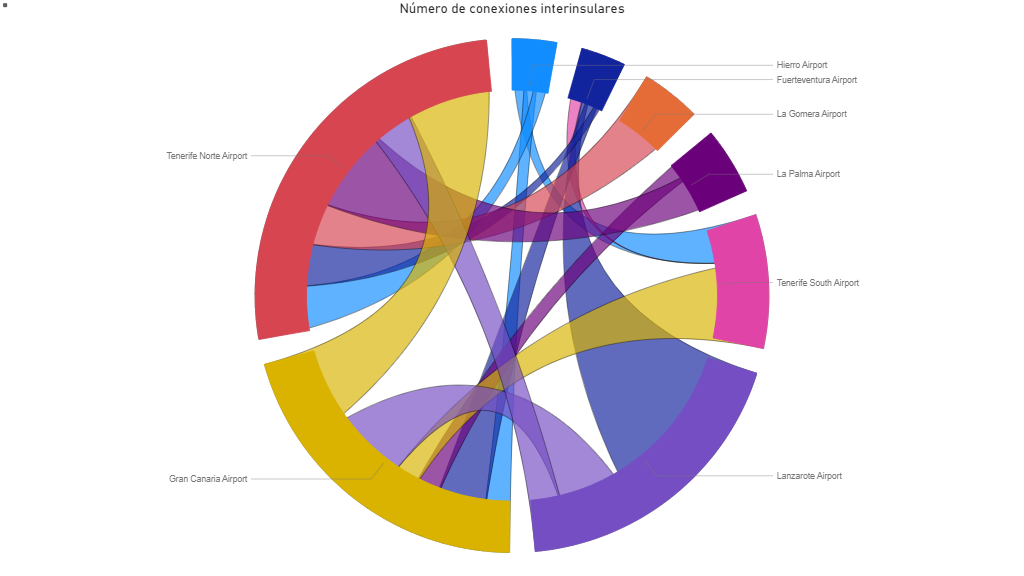
\includegraphics[width=0.8\textwidth]{fotos/cuerda.png}
\caption{Conexiones interinsulares en Canarias.}
\label{fig:cuerdas}
\end{figure}


\section{Gráfico de barras apiladas}

Para mostrar la presencia de las distintas aerolíneas en Canarias, se recurre a un gráfico de barras apiladas. Para hacer un desglose por islas, es necesario crear nuevas medidas en la tabla de rutas: se crean medidas del número de rutas de cada aerolínea con destino en cada isla, con nombres tipo ``VuelosACE'' (para Lanzarote), ``VuelosFTV'' (para Fuerteventura), etc. 
\begin{lstlisting}[style=terminal]
VuelosACE = CALCULATE(COUNT('public routes'[airline_id]), FILTER('public routes', 'public routes'[destination_airport_id] = 1055))
\end{lstlisting}

El resto tienen una estructura completamente análoga, cambiando el ID. Como valores para el gráfico, se pasarán estas medidas, junto con el nombre de las aerolíneas, es decir, la columna ``name'' de la tabla ``airlines''. Con esto, se forma un dataframe que, manipulando un poco en R, da como resultado el gráfico mostrado. El código de R usado es el siguiente: simplemente ordena el eje x (aerolíneas) por cantidad de rutas y ajusta los parámetros del plot haciendo uso de la librería ``ggplot2''. 

\begin{lstlisting}[style=R]
# El codigo siguiente, que crea un dataframe y quita las filas duplicadas, siempre se ejecuta y actua como un preambulo del script:

# dataset <- data.frame(undefined, undefined.1, undefined.2, undefined.3, undefined.4, undefined.5, undefined.6, undefined.7, undefined.8)
# dataset <- unique(dataset)
  
# Pegue o escriba aqui el codigo de script:
library(tidyr)
library(ggplot2)
library(dplyr)
  
data_long <- dataset %>%
  gather(key = "Isla", value = "Vuelos", VuelosACE:VuelosVDE) %>%
  group_by(name) %>%
  mutate(total_vuelos = sum(Vuelos, na.rm = TRUE)) %>%
  ungroup() %>%
  arrange(desc(total_vuelos))

ggplot(data_long, aes(x = factor(name, levels = unique(name)), y = Vuelos, fill = Isla)) +
    geom_bar(stat = "identity") +
    theme_minimal() +
    labs(title = "Presencia de aerolineas en Canarias",
          x = "Aerolinea", y = "Numero de vuelos") +
    theme(axis.text.x = element_text(angle = 45, hjust = 1, size = 8),
          plot.title = element_text(hjust = 0.5)) +
    scale_fill_manual(values = c("VuelosACE" = "#ca3142", "VuelosFTV" = "#009eff", "VuelosLPA" = "#4ad986", "VuelosTFN" = "#a226ff", "VuelosTFS" = "#fe9dff", "VuelosGMZ" = "#ffaa2c", "VuelosSPC" = "yellow", "VuelosVDE" = "#00ffbe"),
                      labels = c("VuelosACE" = "Lanzarote", "VuelosFTV" = "Fuerteventura", "VuelosLPA" = "Gran Canaria", "VuelosTFN" = "Tenerife (norte)", "VuelosTFS" = "Tenerife (sur)", "VuelosGMZ" = "La Gomera", "VuelosSPC" = "La Palma", "VuelosVDE" = "El Hierro"))  
\end{lstlisting}

Este gráfico (figura \ref{fig:barras}) es importante para ver la presencia de las distintas aerolíneas en Canarias. La principal aerolínea es Ryanair, que destaca de forma notable sobre el resto. Esto se debe al gran número de rutas nacionales e internacionales que implementa esta aerolínea en el archipiélago canario. Se puede ver además como de las 10 principales, solo 2 son españolas. Además, se destaca la presencia de una mayoría de aerolíneas que no operan a nivel nacional, aportando solo rutas internacionales.

\begin{figure}[h]
\centering
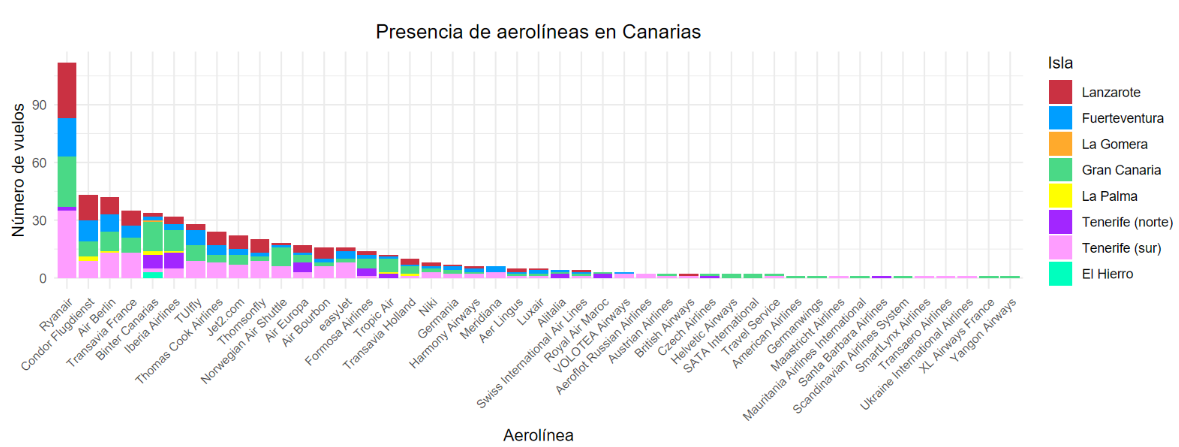
\includegraphics[width=\textwidth]{fotos/barras.png}
\caption{Presencia de aerolíneas en Canarias.}
\label{fig:barras}
\end{figure}

\section{Mapa coroplético}

Este mapa se realizará como visual de \textit{Python}, ya que existen numerosas librerías que permiten la creación de mapas coropléticos de forma muy sencilla. El único cálculo necesario en este caso es el número de vuelos directos a Canarias por país. Para ello, se crea una nueva tabla, ``Vuelos por Pais'', que contiene la magnitud que buscada, así como el país de origen 
\begin{lstlisting}[style=terminal]
Vuelos por Pais = SUMMARIZE(FILTER('public routes', 'public routes'[destination_airport_id] IN {1051, 1052, 1053, 1054, 10551, 1056, 1057, 5659}), 'public airports origen'[country], "Cantidad de Vuelos", COUNT('public routes'[airline_id]))
\end{lstlisting}

Esta tabla tendrá por tanto dos columnas, ``country'' y ``Cantidad de Vuelos''; estos serán los campos a introducir en valores para generar el visual. En cuanto al código python empleado, se usó la librería plotly, que permite la creación de mapas iteractivos. No obstante, \textit{Power BI} no soporta la visualización de estos mapas, por lo que se guarda la representación como imagen plana y se muestra usando matplotlib. A continuación, el código \textit{Python} empleado: 
\begin{lstlisting}[style=python]  
# El codigo siguiente, que crea un dataframe y quita las filas duplicadas, siempre se ejecuta y actua como un preambulo del script:

# dataset = pandas.DataFrame(Cantidad de Vuelos, country)
# dataset = dataset.drop_duplicates()

# Pegue o escriba aqui el codigo de script:

import plotly.express as px
import matplotlib.pyplot as plt
import matplotlib.image as mpimg


fig = px.choropleth(dataset, locations = 'country', locationmode = 'country names',
                    color = "Cantidad de Vuelos", hover_name = 'country', color_continuous_scale = px.colors.sequential.Sunsetdark,
                    title = 'Numero de rutas directas a Canarias por paises')

fig.update_layout(margin = {"r":0, "t":0, "l":0, "b":0},
                  title = {'y':0.87, 'x':0.5, 'xanchor':'center'},
                  coloraxis_colorbar = dict(len=0.7, y=0.5, title="Rutas directas"))

fig.write_image('choropleth_map.png')

img = mpimg.imread('choropleth_map.png')
plt.figure(figsize=(15,10))
plt.imshow(img)
plt.axis('off')
plt.show()
\end{lstlisting}

Esta visualización (figura \ref{fig:coro}) muestra algo curioso: existe un mayor número de conexiones con Reino Unido que con el propio territorio nacional, que presenta un número de conexiones similar al de Alemania. Esto evidencia las fuentes principales del turismo en Canarias y el crecimiento descontrolado de este sector.

\begin{figure}[h]
\centering
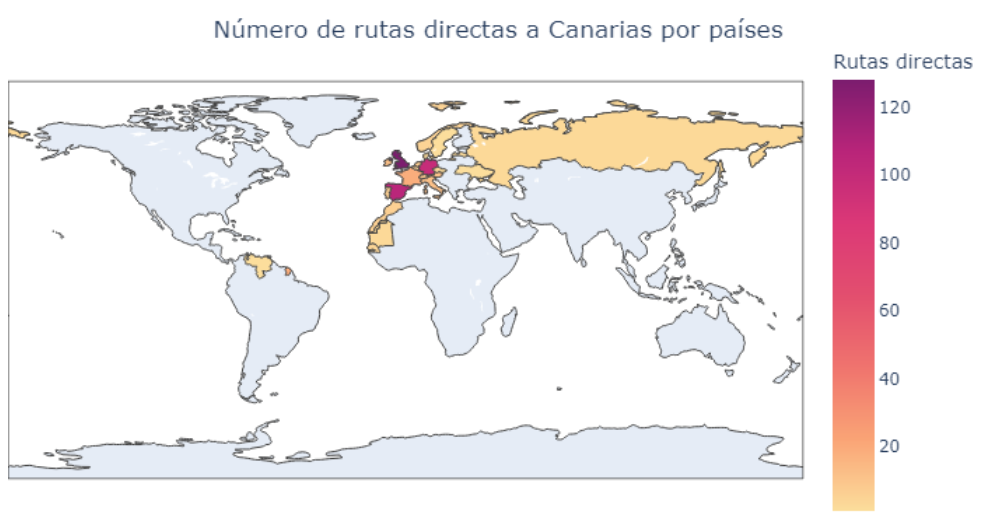
\includegraphics[width=\textwidth]{fotos/coro.png}
\caption{Rutas directas a Canarias por países.}
\label{fig:coro}
\end{figure}

\section{Mapa de flujo}

Para crear este mapa se comienza con un proceso similar al visto para el diagrama de cuerdas: filtrar las rutas. Esta vez, se busca filtrar las rutas con destino Canarias y origen fuera de las islas. Para ello, se crea una nueva tabla, ``RutasFiltradas'',

\begin{lstlisting}[style=terminal]
RutasFiltradas = FILTER('public routes', NOT('public routes'[source_airport_id] IN {1051, 1052, 1053, 1054, 1055, 1056, 1057, 5659}) && 'public routes'[destination_airport_id] IN {1051, 1052, 1053, 1054, 1055, 1056, 1057, 5659})
\end{lstlisting}

La visualización usada es ``Flow Map'' de \textit{Weiwei Cui}, y no se encuentra disponible en los visuales por defecto. Esta representación requiere simplemente de valores de origen y destino para generar las trayectorias o rutas, modificables en color y anchura aportando otros campos como filtros. Los valores de origen y destino se deben dar como puntos (latitud, longitud), por lo que se crean nuevas columnas en la tabla generada para calcular, primero las coordenadas:

\begin{lstlisting}[style=terminal]
LatitudOrigen = RELATED('public airports origen'[latitude])
LongitudOrigen = RELATED('public airports origen'[longitude])
LatitudDestino = RELATED('public airports destino'[latitude])
LongitudDestino = RELATED('public airports destino'[longitude])
\end{lstlisting}

\noindent y posteriormente la concatenación de estas, para obtener el formato esperado por el mapa de flujo

\begin{lstlisting}[style=terminal]
Origen = CONCATENATE(RutasFiltradas[LatitudOrigen], CONCATENATE(", ", RutasFiltradas[LongitudOrigen]))

Destino = CONCATENATE(RutasFiltradas[LatitudDestino], CONCATENATE(", ", RutasFiltradas[LongitudDestino]))
\end{lstlisting}

En este caso, debido al gran volumen de rutas desde la península Ibérica y Reino Unido, escalar las trayectorias resultaba inviable para la correcta visualización del mapa, por lo que se puso una cota superior a este escalado, adecuada para poder visualizar el máximo número de rutas posibles. Esto se consigue ajustando el ancho de las trayectorias: se usa una escala lineal con mínimo 1 y máximo 5. \\

Este mapa, al ser un visual de \textit{Power BI}, permite interacción. De este modo, y para aportar un mayor conocimiento acerca del tráfico aéreo, se muestran los nombres del origen y el destino: al situarse sobre cualquier trayectoria, se pueden ver los distintos puntos de origen que convergen a un mismo destino. Para conseguir esto, se crean dos nuevas columnas, ``NombreOrigen'' y ``NombreDestino'', que relacionan el ID del aeropuerto con su nombre, como se hizo en el diagrama de cuerdas, y se introducen en el apartado ``Tooltips'' del visual: 

\begin{lstlisting}[style=terminal]
NombreOrigen = RELATED('public airports origen'[name])
NombreDestino = RELATED('public airports destino'[name])
\end{lstlisting}

Este gráfico (figura \ref{fig:flow_map}) hace explícita la variedad de conexiones que existen con Canarias, y la distribución de las mismas a lo largo de tres continentes. Si bien el flujo principal proviene de Europa, desde todos los paises de europa occidental y parte de europa del este, también existen rutas hacia el este africano y sudamérica. 

\begin{figure}[H]
\centering
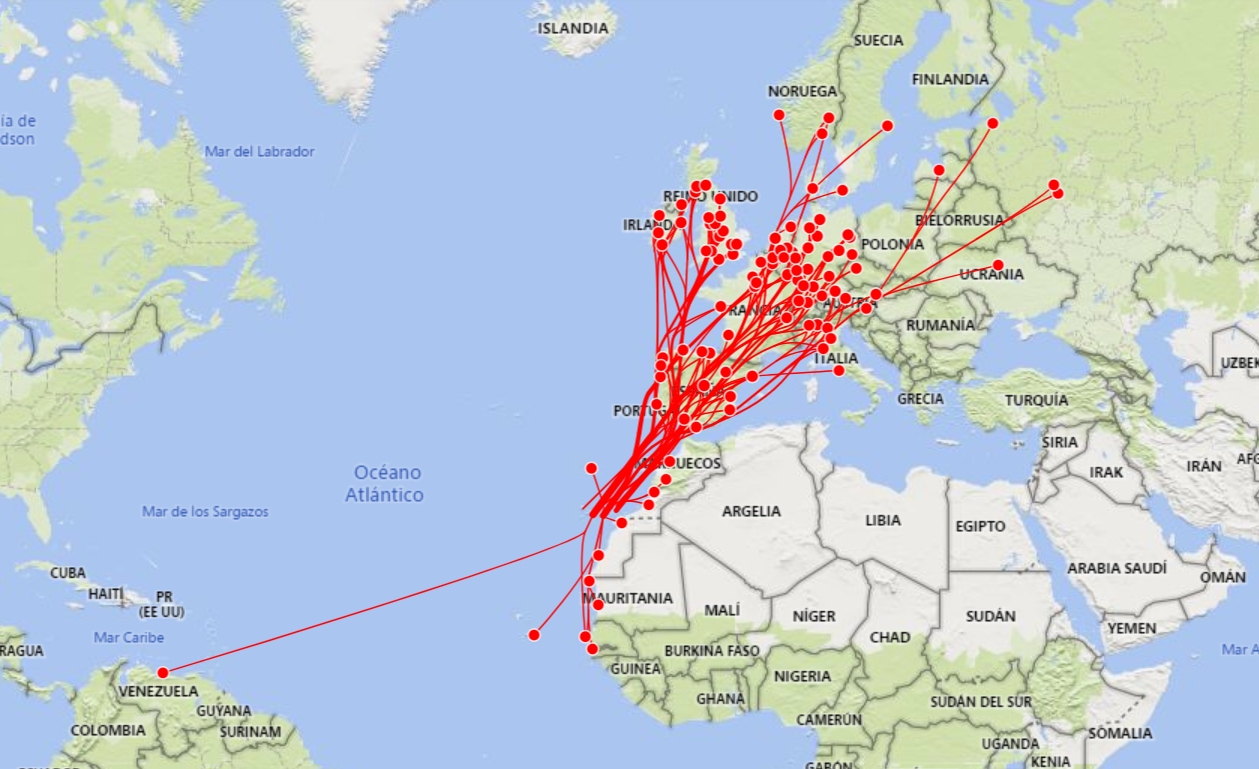
\includegraphics[width=0.73\textwidth]{fotos/flow_map.png}
\caption{Rutas aéreas a Canarias.}
\label{fig:flow_map}
\end{figure}

\section{Resultado final}

A continuación se muestra la composición de los cuatro visuales en un único dashboard (figura \ref{fig:dashboard}). Este dashboard permite una visión global del tráfico aéreo en Canarias, mostrando las conexiones interinsulares, la presencia de las distintas aerolíneas, las rutas directas a Canarias por países y las rutas aéreas a Canarias, arrojando un poco de claridad sobre el insostenible modelo turístico actual del archipiélago.

\begin{figure}[H]
\centering
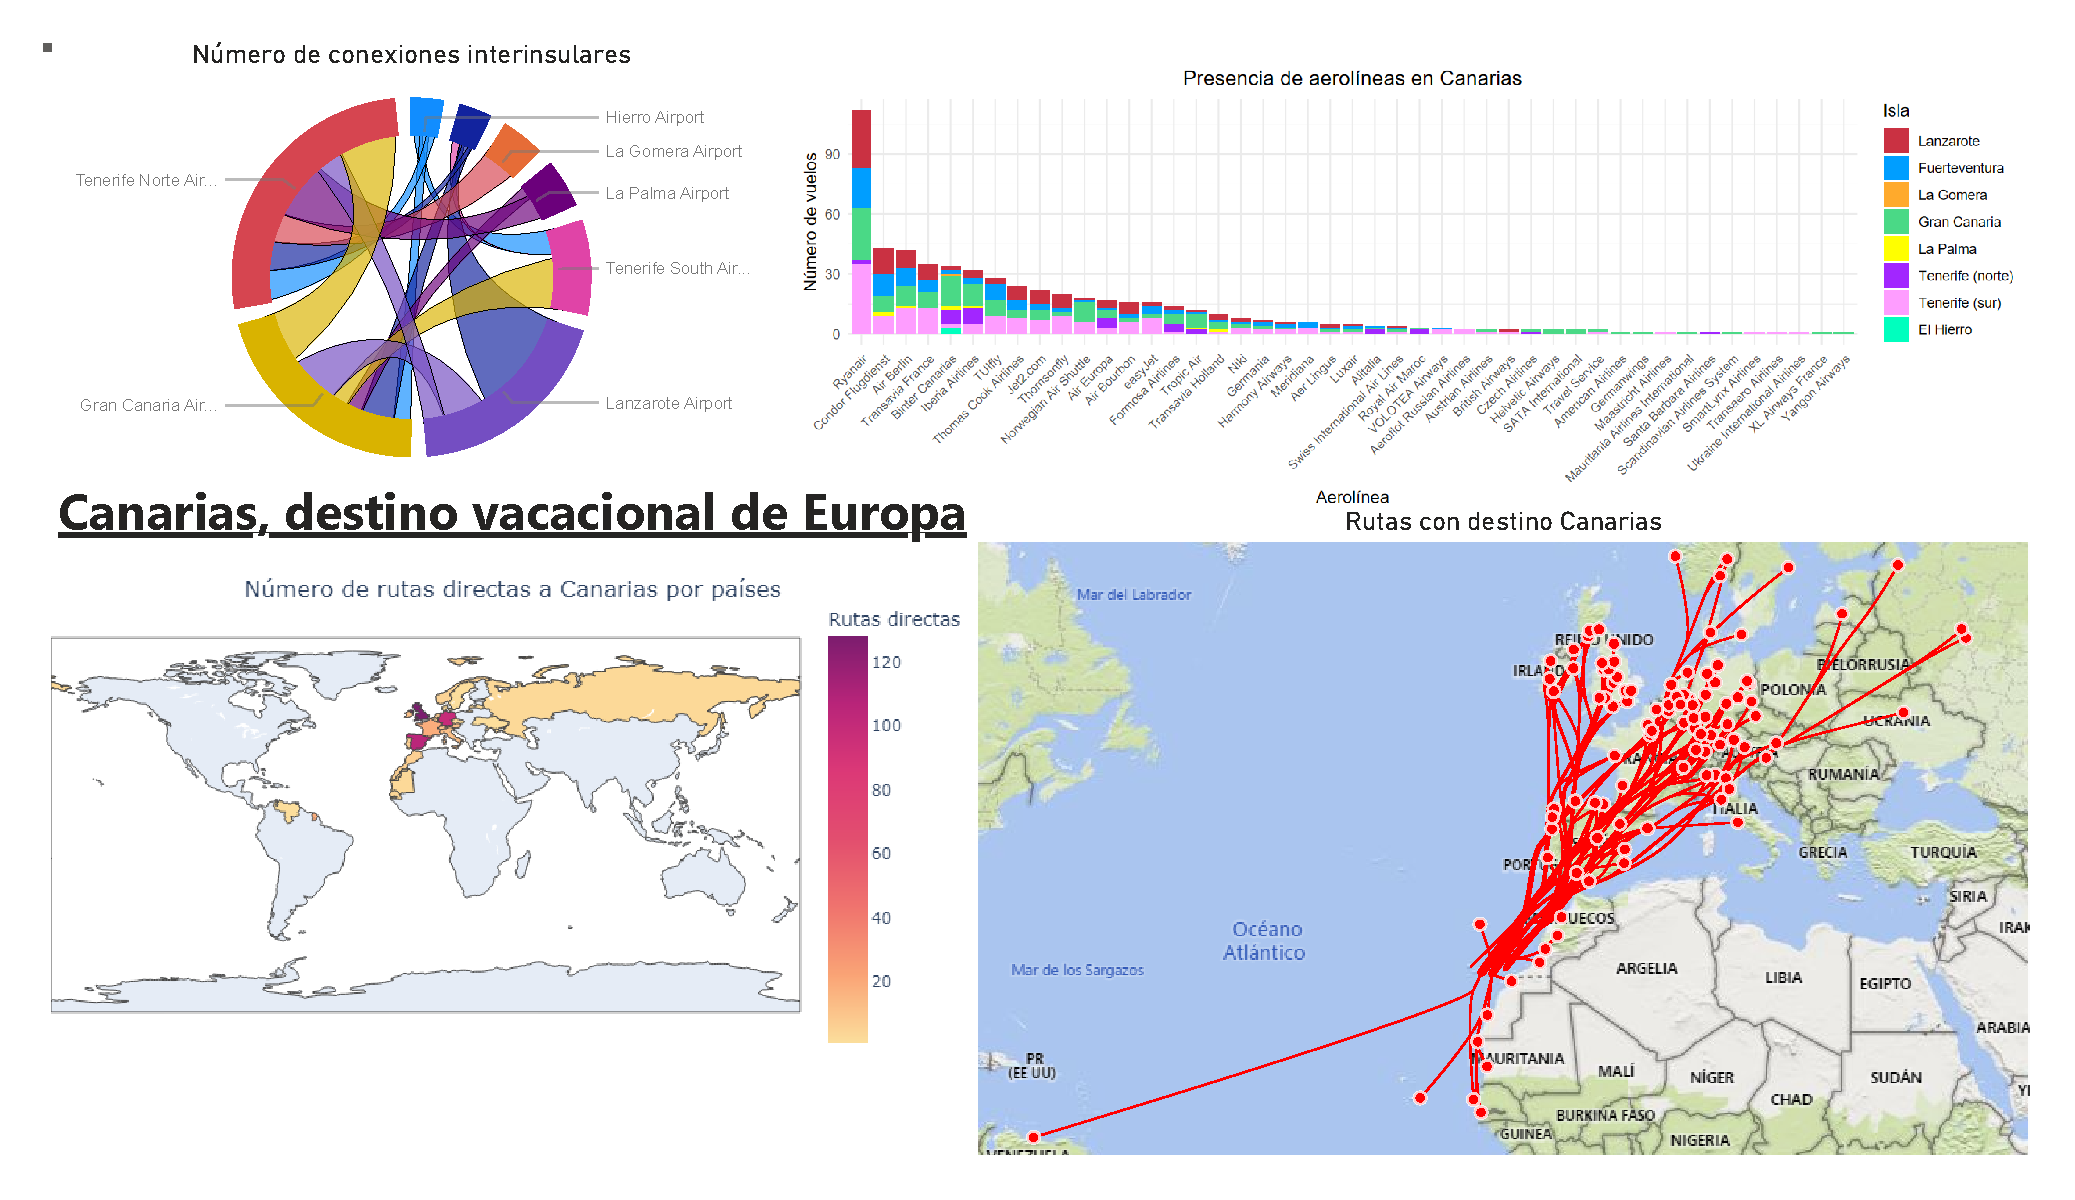
\includegraphics[width=\textwidth]{fotos/PowerBI_LuisArdevol.pdf}
\caption{Canarias, destino vacacional de Europa.}
\label{fig:dashboard}
\end{figure}

\end{document}
